\chapter{Indecidibilità - Il metodo della
diagonalizzazione}

II metodo della diagonalizzazione fu introdotto da Georg Cantor nel 1873 mentre cercava come confrontare gli insiemi infiniti, in particolare come stabilire se, dati due insiemi infiniti, uno sia "più grande" dell'altro.
Cantor osservò che due insiemi finiti hanno la stessa cardinalità se gli elementi dell'uno possono essere messi in corrispondenza uno a uno con quelli dell'altro.
Estese questo concetto agli insiemi infiniti.
Introdusse il metodo della diagonalizzazione per provare che esistono insiemi infiniti di differente cardinalità.
In particolare mostrò che l'insieme $\mathbb{N}$ dei numeri naturali ha cardinalità "inferiore" a quella dell'insieme $\mathbb{R}$ dei numeri reali.

\vspace{5mm}

Il metodo della diagonalizzazione fu successivamente usato per dimostrare che esistono linguaggi non Turing riconoscibili. Il metodo della diagonalizzazione e l'autoreferenzialità sono usati per dimostrare il teorema seguente

\vspace{5mm}

\textbf{Teorema}

Il linguaggio
$A_{T M}=\{\langle M, w\rangle \mid M$ è una macchina di Turing e $M$ accetta $w\}$ non è decidibile.

\subsubsection{Cardinalità}

\textbf{Definizione}

Due insiemi $X$ e $Y$ hanno la stessa cardinalità se esiste una funzione biettiva $f: X \rightarrow Y$ di $X$ su $Y$.

$|X|=|Y| \Leftrightarrow$ esiste una funzione biettiva $f: X \rightarrow Y$

\vspace{5mm}


\textbf{Esempio} $f:\{1,2,5\} \rightarrow\{2,4,7\}$,
dove $f(1)=2, f(2)=4, f(5)=7$, è biettiva

\textbf{Esempio} $f: \mathbb{N} \rightarrow\{2 n \mid n \in \mathbb{N}\}$,
dove $f(n)=2 n$, per ogni $n \in \mathbb{N}$, è biettiva

\vspace{5mm}

\textbf{Esempio (funzione coppia di Cantor)}

Sia $\mathbb{Q}^{+}=\left\{\frac{x}{y} \mid x, y \in \mathbb{N}, y \neq 0\right\}$, la funzione $f: \mathbb{Q}^{+} \rightarrow \mathbb{N}$ definita come segue è biettiva
$$
\begin{aligned}
\forall(x, y) \in \mathbb{N}^{2} \quad f((x, y)) &=\frac{(x+y)(x+y+1)}{2}+x \\
&=\frac{1}{2}\left((x+y)^{2}+3 x+y\right) \in \mathbb{N}
\end{aligned}
$$

\begin{figure}[hbpt!]
    \centering
    \includegraphics[width=7cm]{./Images/8.1.png}
\end{figure}
\FloatBarrier

\subsubsection{Numerabilità}

\textbf{Definizione}

Un insieme $X$ è numerabile se esiste una funzione biettiva $f: \mathbb{N} \rightarrow X \operatorname{di} \mathbb{N}$ su $X .$
Un insieme $X$ è enumerabile se esiste una funzione biettiva calcolabile $f: \mathbb{N} \rightarrow X$ di $\mathbb{N}$ su $X$.
Un insieme $X$ è contabile se è finito o numerabile.


Esempio L'insieme dei numeri pari è numerabile.

Esempio $\mathbb{Q}^{+}=\left\{\frac{x}{y} \mid x, y \in \mathbb{N}, y \neq 0\right\}, \mathbb{N}^{2}$ sono numerabili.

\vspace{5mm}

$\mathbb{R}$ non è numerabile.
Non esiste nessuna funzione biettiva di $\mathbb{N}$ sull'insieme $\mathbb{R}$ dei numeri reali.

Nella dimostrazione che segue potremmo anche limitarci a considerare i numeri reali nell'intervallo ] 0,1 [ perché questo insieme ha cardinalità non superiore a $\mathbb{R}$.


\subsubsection{Idea della prova (metodo della diagonalizzazione)} 
Supponiamo per assurdo che esista una funzione biettiva $f$ di $\mathbb{N}$ su $\mathbb{R}$. Allora possiamo costruire la tabella:

\begin{center}
\begin{tabular}{c|ccccc}
$n$ & & & & $f(n)$ & \\
\hline 1 & $d_{1,1}$ & $d_{1,2}$ & $\ldots$ & $\ldots$ & $\ldots$ \\
2 & $d_{2,1}$ & $d_{2,2}$ & $\ldots$ & $\ldots$ & $\ldots$ \\
$.$ & $\ldots$ & $\ldots$ & $\ldots$ & $\ldots$ & $\ldots$ \\
$.$ & $\ldots$ & $\ldots$ & $\ldots$ & $\ldots$ & $\ldots$ \\
$i$ & $d_{i, 1}$ & $d_{i, 2}$ & $\ldots$ & $\ldots$ & $\ldots$ \\
$.$ & $\ldots$ & $\ldots$ & $\ldots$ & $\ldots$ & $\ldots$ \\
$.$ & $\ldots$ & $\ldots$ & $\ldots$ & $\ldots$ & $\ldots$
\end{tabular}
\end{center}


dove $d_{1,1} d_{1,2} \ldots$ è la parte decimale del numero reale $f(1)$, $d_{2,1} d_{2,2} \ldots$ è la parte decimale del numero reale $f(2)$ e in generale $d_{i, 1} d_{i, 2} \ldots$ è la parte decimale del numero reale $f(i)$.

\vspace{5mm}


quindi $f(1)=r_{1}, d_{1,1} d_{1,2} \ldots, f(2)=r_{2}, d_{2,1} d_{2,2} \ldots \mathrm{e}$ in generale $f(i)=r_{i}, d_{i, 1} d_{i, 2} \ldots .$

Le cifre sulla diagonale di questa matrice $d_{1,1} d_{2,2} \ldots$ definiscono un numero reale $r=0, d_{1,1} d_{2,2} \ldots$.

II numero reale $0, d_{1,1}^{\prime} d_{2,2}^{\prime} \ldots$ che si ottiene scegliendo in ogni posizione (della parte decimale) una cifra diversa dalla corrispondente cifra in $r$ non è immagine di nessun intero positivo (non può essere $f(1)$ perché $d_{1,1}^{\prime} \neq d_{1,1}$, non può essere $f(2)$ perché $\left.d_{2,2}^{\prime} \neq d_{2,2}, \ldots . .\right)$

\subsubsection{Cardinalità}
\begin{itemize}
    \item $|X| \leq|Y| \Leftrightarrow$ esiste una funzione iniettiva $f: X \rightarrow Y$
    \item $|X| \leq|Y|,|X| \neq|Y| \Rightarrow|X|<|Y|$
    \item $|X| \leq|Y|,|Y| \leq|X| \Rightarrow|X|=|Y|$
\end{itemize}

$n \in \mathbb{N} \rightarrow n \in \mathbb{R}$ è una funzione iniettiva di $\mathbb{N}$ in $\mathbb{R}$. Quindi| $|\mathbb{N}| \leq|\mathbb{R}| .$


Non esiste nessuna funzione biettiva di $\mathbb{N}$ sull'insieme $\mathbb{R}$ dei numeri reali. Quindi $|\mathbb{N}| \neq|\mathbb{R}|, \mathbb{N}$ e $\mathbb{R}$ non hanno la stessa cardinalità. Quindi da $|\mathbb{N}| \leq|\mathbb{R}|$ e $|\mathbb{N}| \neq|\mathbb{R}|$ deduciamo $|\mathbb{N}|<|\mathbb{R}|$.


Nota. Lo stesso metodo può essere usato per mostrare che per ogni insieme $S$ risulta $|S|<|\mathcal{P}(S)|$.

\subsubsection{Il Metodo della diagonalizzazione per provare che esistono
linguaggi non Turing riconoscibili}

E' possibile usare il metodo della diagonalizzazione per provare che esistono linguaggi che non sono Turing riconoscibili.
La prova consiste nel provare le affermazioni seguenti:
\begin{itemize}
    \item Dato un alfabeto $\Sigma$, l'insieme $\Sigma^{*}$ è numerabile.
    \item L'insieme delle codifiche delle macchine di Turing, e quindi l'insieme delle macchine di Turing è numerabile.
Nota: la codifica di una Macchina di Turing è una stringa.
    \item L'insieme dei linguaggi Turing riconoscibili è numerabile. Nota: a ogni linguaggio Turing riconoscibile è associata (la codifica di) una macchina di Turing.
    \item L'insieme dei linguaggi sull'alfabeto $\Sigma$ ha cardinalità| maggiore del numerabile.
\end{itemize}

\subsubsection{Numerabilità dell'insieme delle parole}

$\Sigma^{*}$ è numerabile

\vspace{5mm}

\textbf{Idea della dimostrazione:}

Provare che $|\mathbb{N}| \leq\left|\Sigma^{*}\right|$ e poi che $\left|\Sigma^{*}\right| \leq|\mathbb{N} \times \mathbb{N}||=| \mathbb{N} \mid$

\subsubsection{Ordine radix}

\textbf{Definizione}

Sia $\Sigma=\left\{a_{1}, \ldots, a_{k}\right\}$ un alfabeto e sia $a_{1}<a_{2}<\ldots<a_{k}$ un ordinamento degli elementi di $\Sigma$. Siano $x, y \in \Sigma^{*}$.

Diremo che $x \leq y$ rispetto all'ordine radix se $x$ e $y$ verificano una delle condizioni seguenti:
\begin{enumerate}
    \item $|x|<|y|$.
    \item $|x|=|y| e x=z a x^{\prime}, y=z b y^{\prime}$, con $z, x^{\prime}, y^{\prime} \in \Sigma^{*} \mid, a, b \in \Sigma e a \leq b$.
\end{enumerate}

In "Introduzione alla teoria della computazione", l'ordine radix è chiamato ordine per lunghezza.

\subsubsection{Enumerazione delle stringhe}

L'ordinamento radix produce una corrispondenza biunivoca tra $\mathbb{N}$ e $\Sigma^{*}$ che permette di enumerare le stringhe:

$w_{0}=\epsilon, w_{1}=a_{1}, w_{2}=a_{2}, \ldots$,

Ad esempio, se $\Sigma=\{a, b\}$, la sequenza è
$$
\epsilon, a, b, a a, a b, b a, b b, \ldots,
$$
e $w_{1}=a, w_{5}=b a, w_{8}=?$

\subsubsection{Non numerabilità dell'insieme dei linguaggi}

Sia $\Sigma^{*}=\{w_{0}, w_{1}, \ldots,\}$,

Sia $\mathcal{B}$ l'insieme delle sequenze binarie infinite cioè delle sequenze infinite di 0 e 1 .

È possibile associare a ogni linguaggio $L$ una sequenza infinita $s_{L}$ (la sequenza caratteristica di $L$ ) così definita:

\vspace{5mm}


\begin{center}
    il bit i-esimo di $s_{L}$ è 1 se l'i-esima stringa wi è in $L$, il bit i-esimo di $s_{L}$ è 0 se $w_{i} \notin L$.
\end{center}

\vspace{5mm}

L'applicazione $f: \mathcal{P}\left(\Sigma^{*}\right) \rightarrow \mathcal{B}$ definita da $f(L)=s_{L}$ è biettiva.

\subsubsection{Non numerabilità dell'insieme delle sequenze binarie}

L'insieme $\mathcal{B}$ non è numerabile.

\vspace{5mm}

\textbf{Idea della prova (metodo della diagonalizzazione).}

Mostriamo che non esiste nessuna funzione biettiva di $\mathbb{N}$ sull'insieme $\mathcal{B}$ delle sequenze binarie infinite. Supponiamo per assurdo che esista una funzione biettiva $f$ di $\mathbb{N}$ su $\mathcal{B}$.
Allora possiamo costruire la tabella:

\vspace{5mm}

\begin{center}
\begin{tabular}{c|ccccc}
$n$ & & & & $f(n)$ & \\
\hline 1 & $d_{1,1}$ & $d_{1,2}$ & $\ldots$ & $\ldots$ & $\ldots$ \\
2 & $d_{2,1}$ & $d_{2,2}$ & $\ldots$ & $\ldots$ & $\ldots$ \\
$.$ & $\ldots$ & $\ldots$ & $\ldots$ & $\ldots$ & $\ldots$ \\
$.$ & $\ldots$ & $\ldots$ & $\ldots$ & $\ldots$ & $\ldots$ \\
$i$ & $d_{i, 1}$ & $d_{i, 2}$ & $\ldots$ & $\ldots$ & $\ldots$ \\
$.$ & $\ldots$ & $\ldots$ & $\ldots$ & $\ldots$ & $\ldots$ \\
$.$ & $\ldots$ & $\ldots$ & $\ldots$ & $\ldots$ & $\ldots$
\end{tabular}
\end{center}

\vspace{5mm}

dove $d_{1,1} d_{1,2} \ldots$ è la sequenza binaria infinita associata a $f(1)$, $d_{2,1} d_{2,2} \ldots$ è la sequenza binaria infinita associata a $f(2)$ e in generale $d_{i, 1} d_{i, 2} \ldots$ è la sequenza binaria infinita associata a $f(i)$.

\vspace{5mm}

Le cifre sulla diagonale di questa matrice $d_{1,1} d_{2,2} \ldots$ definiscono una sequenza binaria infinita $s$.

La sequenza binaria infinita $\bar{d}_{1,1} \bar{d}_{2,2} \ldots$ che si ottiene scegliendo in ogni posizione il complemento della corrispondente cifra in $s$ non è immagine di nessun intero positivo (non può essere $f(1)$ perché $\bar{d}_{1,1} \neq d_{1,1}$, non può essere $f(2)$ perché $\left.\bar{d}_{2,2} \neq d_{2,2}, \ldots . .\right)$

\subsubsection{Non numerabilità dell'insieme dei linguaggi}

L'insieme $\mathcal{P}\left(\Sigma^{*}\right)$ dei linguaggi su $\Sigma$ non è numerabile. 

\vspace{5mm}

\textbf{Dimostrazione}

Esiste un'applicazione biettiva $f$ di $\mathcal{P}\left(\Sigma^{*}\right)$ in $\mathcal{B}$, quindi $|\mathcal{B}|=\left|\mathcal{P}\left(\Sigma^{*}\right)\right|$.

Poiché, come abbiamo provato, $\mathcal{B}$ non è numerabile, concludiamo che $\mathcal{P}\left(\Sigma^{*}\right)$ non è numerabile.

\subsubsection{Esistono linguaggi non Turing riconoscibili}

La funzione $h: \Sigma^{*} \rightarrow \mathcal{P}\left(\Sigma^{*}\right)$, dove $h(w)=\{w\}$, è iniettiva. Quindi
$\mid\left\{L \subseteq \Sigma \mid L\right.$ è Turing riconoscibile $\}|\leq| \Sigma^{*}|<| \mathcal{P}\left(\Sigma^{*}\right) \mid$.
Possiamo concludere che l'insieme dei linguaggi Turing riconoscibili è (al più) numerabile ma l'insieme di tutti i linguaggi ha cardinalità maggiore del numerabile.

\vspace{5mm}

\textbf{Corollario}

Esistono linguaggi che non sono Turing riconoscibili.

\subsubsection{Non numerabilità dell'insieme dei linguaggi}

L'insieme $\mathcal{P}\left(\Sigma^{*}\right)$ dei linguaggi su $\Sigma$ non è numerabile.

\vspace{5mm}

\textbf{(Seconda) Dimostrazione}

Supponiamo per assurdo che $\mathcal{P}\left(\Sigma^{*}\right)$ sia numerabile.
Quindi esiste un'applicazione biettiva $h$ di $\mathbb{N}$ in $\mathcal{P}\left(\sum^{*}\right)$.

Sia $L_{0}, L_{1}, \ldots$ la lista dei linguaggi, cioè degli elementi di
$\mathcal{P}\left(\Sigma^{*}\right)$, dove $L_{0}=h(0), L_{1}=h(1)$ e in generale $L_{i}=h(i)$.

Anche $\Sigma^{*}$ è enumerabile, sia $g$ una biezione $d i \mathbb{N}$ in $\Sigma^{*}$ e siano $w_{0}, w_{1}, \ldots$ gli elementi di $\Sigma^{*}$, con $w_{i}=g(i)$.

\vspace{5mm}

\begin{center}
    \begin{tabular}{c|ccccc} 
& $w_{0}$ & $w_{1}$ & $\ldots$ & $w_{j}$ & \\
\hline$L_{0}$ & 0 & 1 & $\ldots$ & 0 & $\ldots$ \\
$L_{1}$ & 1 & 1 & $\ldots$ & 1 & $\ldots$ \\
$L_{2}$ & 0 & 0 & $\ldots$ & 1 & $\ldots$ \\
$\cdot$ & $\ldots$ & $\ldots$ & $\ldots$ & $\ldots$ & $\ldots$ \\
$L_{i}$ & 1 & 0 & $\ldots$ & 0 & $\ldots$ \\
$\cdot$ & $\ldots$ & $\ldots$ & $\ldots$ & $\ldots$ & $\ldots$ \\
$\cdot$ & $\ldots$ & $\ldots$ & $\ldots$ & $\ldots$ & $\ldots$
\end{tabular}

\end{center}

\vspace{5mm}

La riga corrispondente ad $L_{i}$ è la sequenza caratteristica di $L_{i}$. Scriviamo 1 all'incrocio tra la riga $L_{i}$ e la colonna $w_{j}$ se $w_{j} \in L_{i}$, altrimenti scriviamo 0 .

\vspace{5mm}

Definiamo L:
$$
\forall i \geq 0 \quad w_{i} \in L \Leftrightarrow w_{i} \notin L_{i}
$$
$L \in \mathcal{P}\left(\Sigma^{*}\right)$ ma per ogni $i \geq 0, L \neq L_{i} .$

Infatti, sia $h$ tale che $L=L_{h}$. La domanda "wh $\in L$ ?" conduce a una contraddizione.

Assumiamo $w_{h} \in L$. Per la definizione di $L$ deve essere $w_{h} \notin L_{h} .$ Ma per ipotesi $L=L_{h}$, assurdo.

Assumiamo $w_{h} \notin L$. Per la definizione di $L$ deve essere $w_{h} \in L_{h}$. Ma per ipotesi $L=L_{h}$, assurdo.

\section{La gerarchia di Chomsky -
Parte II}

\subsubsection{Grammatica di tipo 0}

Una grammatica (di tipo 0 o a struttura di frase) $G$, è una quadrupla $G=(V, T, P, S)$ dove:
\begin{itemize}
    \item V: Insieme finito di variabili (dette anche non terminali o categorie sintattiche). Ogni variabile rappresenta un linguaggio.
    \item T: Insieme finito di simboli terminali (o alfabeto dei terminali). È l'alfabeto delle parole del linguaggio da definire. $T \cap V=\emptyset$.
    \item P: Insieme fin ito delle produzioni. Ogni produzione ha la forma $\alpha \rightarrow \beta$, dove $\alpha \in(V \cup T)^{+} e \beta \in(V \cup T)^{*}$.
    \item S: Una variabile, detta simbolo iniziale (o start symbol), che rappresenta il linguaggio definito dalla grammatica.
\end{itemize}

\subsubsection{Grammatica di tipo 1}
Una grammatica $G=(V, T, P, S)$ è una grammatica di tipo 1 o dipendente dal contesto se ogni $\alpha \rightarrow \beta \in P$ è tale che $\alpha \in(V \cup T)^{+}, \beta \in(V \cup T)^{+}$e il lato destro di ogni produzione ha lunghezza almeno pari al lato sinistro
$$
\forall \alpha \rightarrow \beta \in P \quad|\beta| \geq|\alpha|
$$
In più permettiamo che $S \rightarrow \epsilon$ sia in $P$ a condizione che $S$ non compaia alla destra di nessuna produzione.

\subsubsection{Grammatica di tipo 2}

Una grammatica $G=(V, T, P, S)$ è una grammatica di tipo 2 se ogni $\alpha \rightarrow \beta \in P$ è tale che $\alpha \in V$ e $\beta \in(V \cup T)^{+}$cioè ogni produzione ha la forma $A \rightarrow \beta$, dove $A$ è una variabile e $\beta$ è una stringa non vuota di variabili e terminali.
In più permettiamo che $S \rightarrow \epsilon$ sia in $P$ a condizione che $S$ non compaia alla destra di nessuna produzione.

\vspace{5mm}

\textbf{Nota.} Le grammatiche di tipo 2 e le grammatiche context-free sono computazionalmente equivalenti: ogni grammatica di tipo 2 è una grammatica context-free e se $G$ è una grammatica context-free esiste una grammatica $G^{\prime}$ di tipo 2 tale che $L(G)=L\left(G^{\prime}\right)$.


\subsubsection{Grammatica di tipo 3}

Una grammatica $G=(V, T, P, S)$ è una grammatica di tipo 3 o regolare se ogni $\alpha \rightarrow \beta \in P$ è tale che $\alpha \in V$ e $\beta \in T \cup(T \cdot V)$, cioè se ogni produzione è della forma $A \rightarrow a B$ o $A \rightarrow a$, dove $A, B$ sono variabili e a è un terminale.

In più permettiamo che $S \rightarrow \epsilon$ sia in $P$ a condizione che $S$ non compaia alla destra di nessuna produzione.

\subsubsection{Riassumendo}

Una grammatica $G=(V, T, P, S)$, con $V, T$ insiemi finiti e disgiunti, $S \in V$ è
\begin{itemize}
    \item di tipo 1 se ogni produzione in $P$ ha la forma $\alpha \rightarrow \beta$, $\alpha, \beta \in(V \cup T)^{+} \mathrm{e}|\beta| \geq|\alpha| .$
    \item di tipo 2 se ogni produzione in $P$ ha la forma $A \rightarrow \beta$, con $A \in V e \beta \in(V \cup T)^{+}$
    \item di tipo 3 se ogni produzione in $P$ ha la forma $A \rightarrow a B$ o $A \rightarrow a$, dove $A, B$ sono variabili e a è un terminale.
\end{itemize}

In più permettiamo che $S \rightarrow \epsilon$ sia in $P$ a condizione che $S$ non compaia alla destra di nessuna produzione.


\subsubsection{Teorema (Gerarchia di grammatiche)}
La classe delle grammatiche di tipo i include strettamente quella delle grammatiche di tipo $i+1,0 \leq i \leq 2$.

\subsubsection{Gerarchia di Chomsky}

Un linguaggio $L$ è di tipo i se esiste una grammatica $G$ di tipo i tale che $L=L(G)$.


Otteniamo quattro classi di linguaggi, i linguaggi di tipo 0,1 , 2,3 . Le quattro classi formano la
Gerarchia di Chomsky

\subsubsection{Linguaggi di tipo 0}

Le grammatiche di tipo 0 sono le grammatiche che non hanno senza alcuna restrizione sulla forma delle produzioni.
Un linguaggio $L$ è di tipo 0 se esiste una grammatica $G$ di tipo 0 tale che $L(G)=L$.

Sia $L$ di tipo 0 . È possibile dimostrare che esiste una macchina di Turing non deterministica $M$ che lo riconosce, cioè tale che $L=L(M)$.
Viceversa, data una macchina di Turing $M$ è possibile dimostrare che esiste una grammatica $G$ di tipo 0 tale che $L(G)=L(M)$

Quindi la classe dei linguaggi di tipo 0 coincide con la classe dei linguaggi Turing riconoscibili.

\subsubsection{Linguaggi di tipo 1 o dipendenti dal contesto}

Le grammatiche di tipo 1 sono le grammatiche in cui il lato destro di ogni produzione ha lunghezza almeno pari al lato sinistro (a parte eventualmente la produzione $S \rightarrow \epsilon$ ).

Un linguaggio $L$ è di tipo 1 se esiste una grammatica $G$ di tipo 1 tale che $L(G)=L$.

\vspace{5mm}

\textbf{Teorema}

I linguaggi di tipo 1 sono decidibili.

Nota. La MT che decide il linguaggio usa implicitamente come sottoprogramma una TM che decide
$A_{C S G}=\{\langle G, w\rangle \mid G$ è di tipo 1 e $w \in L(G)\}$

\subsubsection{Decidibilità dei linguaggi context-sensitive}


(Idea della prova). Sia $G=(V, \Sigma, P, S)$ una grammatica di tipo 1 e sia $w \in L(G), w \neq \epsilon$. Quindi $S \underset{G}{\Rightarrow} w$.

Ogni derivazione diretta in $S \xRightarrow[G]{*} w$ sostituisce una stringa $\alpha$ con una stringa $\beta$ più lunga.

Quindi in ognuna di tali derivazioni dirette compaiono solo stringhe di lunghezza minore o uguale alla lunghezza di $w$.

\vspace{5mm}

Ad esempio sia $G=(V, \Sigma, P, S)$, dove $V=\{S, B\}, T=\{a, b, c\}$ e $P$ consiste nelle seguenti produzioni
$S \rightarrow a S B c \mid a b c, \quad c B \rightarrow B c, \quad b B \rightarrow b b$
Sappiamo che $L(G)=\left\{a^{n} b^{n} c^{n} \mid n \geq 1\right\}$
$S \Rightarrow a S B C \Rightarrow a a b c B C \Rightarrow a a b B C C \Rightarrow a a b b c c$

\vspace{5mm}

(Idea della prova). Sia $G=(V, \Sigma, P, S)$ una grammatica di tipo 1 e sia $w \in \Sigma^{+}$con $|w|=n$.
Risulta $w \in L(G)$ se e solo se esiste una sequenza $\alpha_{1}, \alpha_{2}, \ldots, \alpha_{k}$ di stringhe in $\bigcup_{t=1}^{n}\left(\sum \cup V\right)^{t}$ tali che $\alpha_{1}=S, \alpha_{k}=w$ e $\alpha_{i} \xRightarrow[G]{} \quad \alpha_{i+1}, i=1, \ldots, k-1$
ovvero
$$
S=\alpha_{1} \xRightarrow[G]{} \alpha_{2} \ldots \alpha_{k-1} \xRightarrow[G]{} \alpha_{k}=w
$$

\vspace{5mm}

Prova (cenni). Sia $G=(V, \Sigma, P, S)$ una grammatica di tipo 1 per $L$. Sia $M_{G}$ una MT definita come segue $\left(M_{G}\right.$ ha una copia di $G$ memorizzata).
$M_{G}="$ Su input $w \in \Sigma^{*}$ :
\begin{enumerate}
    \item Verifica se $w=\epsilon$. In tal caso accetta se $S \rightarrow \epsilon \in P ;$ altrimenti rifiuta.
    \item Se $w \neq \epsilon$, conta i caratteri di $w$. Sia $n=|w|$.
    \item Costruisce un grafo orientato i cui vertici sono le stringhe di $(V \cup \Sigma)^{+}$ di lunghezza minore di o uguale a $n$. Pone un arco da $\alpha$ a $\beta$ se $\alpha \underset{G}{\stackrel{}{\Rightarrow}} \beta$.
    \item Verifica se c'è un cammino dal vertice (per) $S$ al vertice (per) $w$. In caso affermativo accetta; altrimenti rifiuta.
\end{enumerate}
$M_{G}$ decide $L$.
Infatti $w \in L(G)$ se e solo se c'è un cammino dal vertice (per) $S$ al vertice (per) $w$.

Esistono algoritmi per decidere se esiste un tale cammino.

\subsubsection{La gerarchia di Chomsky}

Prova alternativa (Cenni). 
Sia $G=(V, \Sigma, P, S)$ una grammatica di tipo $1 .$
Sia $k=|V \cup \Sigma|$. Per ogni $n \geq 0$, l'insieme delle stringhe di lunghezza al più $n$ è un insieme finito e risulta
$$
\left|\left\{\gamma \in(V \cup \Sigma)^{*}|| \gamma \mid \leq n\right\}\right|=\sum_{j=0}^{n} k^{j}=\ell
$$

\vspace{5mm}

Sia $w \in \Sigma^{*} \mathrm{e}|w|=n$. Consideriamo la seguente successione $\mathcal{S}^{(n)}$ di insiemi
$$
\begin{aligned}
A_{0} &=\{S\} \\
A_{i+1} &=A_{i} \cup\left\{\beta\left|\alpha \in A_{i}, \alpha \Rightarrow \beta,\right| \beta \mid \leq n\right\}, \quad i \geq 0
\end{aligned}
$$
Per ogni $j>0, A_{j} \backslash\{S\}$ è l'insieme delle stringhe di lunghezza al più $n$ derivabili in $j$ passi. Quindi $w \in L(G)$ se e solo se $w \in A_{j}$ per qualche $j>0$.
Si noti che $A_{i} \subseteq A_{i+1}$, che se $A_{i}=A_{i+1}$ allora $A_{i}=A_{i+h}$, per ogni $h, h \geq 0$.
La successione in esame è superiormente limitata da $A_{\ell}$, che contiene al massimo $\ell$ stringhe.

\vspace{5mm}

Sia $G=(V, \Sigma, P, S)$ una grammatica di tipo 1 per $L .$ Sia $M_{G}$ una $M T$ definita come segue $\left(M_{G}\right.$ ha una copia di $G$ memorizzata $)$. $M_{G}=" S u$ input $w \in \Sigma^{*}:$
\begin{enumerate}
    \item Conta i caratteri di $w$. Sia $n=|w|$.
    \item Costruisce la successione finita $\mathcal{S}^{(n)}$ degli insiemi finiti $A_{j}$.
    \item Verifica se $w$ appartiene a uno di questi insiemi $A_{j}$.
    \item In caso affermativo accetta; altrimenti rifiuta.
\end{enumerate}

Ricordiamo che il nome di "grammatica dipendente dal contesto" deriva dal fatto che per ogni $G$ di tipo 1 , esiste $G^{\prime}$ tale che $L(G)=L\left(G^{\prime}\right)$ e in cui le produzioni hanno la forma
$$
\alpha_{1} A \alpha_{2} \rightarrow \alpha_{1} \beta \alpha_{2}
$$
dove $A$ è una variabile, $\alpha_{1}, \alpha_{2}, \beta$ sono stringhe di variabili e terminali e $\beta \neq \epsilon$. (Quindi anche $G^{\prime}$ è di tipo 1 ).

Cioè è possibile sostituire $A$ con $\beta$ ma solo se $A$ appare nella stringa in un contesto particolare.
Alcuni autori adottano come definizione quella in cui le produzioni hanno questo secondo vincolo. Ma la prima formulazione ha il vantaggio di mettere in evidenza la decidibilità dei linguaggi generati da queste grammatiche.

\vspace{5mm}

Conseguenza del precedente teorema:

\vspace{5mm}
\begin{center}
    I linguaggi di tipo 2 sono decidibili.
\end{center}
\vspace{5mm}


La decidibilità dei linguaggi context-free può essere provata direttamente.

\subsubsection{Definizione di forma normale di Chomsky}

Una grammatica context-free $G=(V, \Sigma, P, S)$ è in forma normale di Chomsky (o in CNF) se ogni sua produzione ha la forma
\begin{enumerate}
    \item $A \rightarrow B C$ con $A, B, C \in V$,
    \item $A \rightarrow a \operatorname{con} A \in V$ e $a \in \Sigma$,
    \item $S \rightarrow \epsilon$
\end{enumerate}

Inoltre, se $S \rightarrow \epsilon$ è in $P$, allora $B, C \in V \backslash\{S\}$ in (1).

\vspace{5mm}

\textbf{Teorema}

Per ogni grammatica context-free $G$ esiste una grammatica $G^{\prime}$ tale che $L\left(G^{\prime}\right)=L(G)$ e $G^{\prime}$ è in forma normale di Chomsky.

\vspace{5mm}

\textbf{Proposizione}

Se $G=(V, \Sigma, P, S)$ è una grammatica context-free in forma normale di Chomsky e w è una stringa in $L(G)$ di lunghezza $n \geq 1$, allora ogni derivazione di $w$ richiede esattamente $2 n-1$ passi.

\vspace{5mm}

$A_{C F G}=\{\langle G, w\rangle \mid G$ è una CFG che genera la stringa $w\} .$

Una TM $S$ per $A_{C F G}:$

\vspace{5mm}

$S="$ Su input $\langle G, w\rangle$, dove $G$ è una CFG e $w$ è una stringa:
\begin{enumerate}
    \item Converte $G$ in una grammatica equivalente in forma normale di Chomsky.
    \item Lista tutte le derivazioni di $2 n-1$ passi, dove $n$ è la lunghezza di $w$; tranne se $n=0$, in tal caso lista tutte le derivazioni di un passo.
    \item Se una di tali derivazioni genera $w$, accetta; altrimenti, rifiuta."
$S$ è un decider e $L(S)=A_{C F G}$.
\end{enumerate}

\vspace{5mm}

\textbf{Teorema}

Ogni linguaggio context-free è decidibile.

\vspace{5mm}

Sia $A$ un $C F L$. Una (cattiva) idea per mostrare che $A$ è decidibile è quella di convertire un PDA per A direttamente in una TM.
Invece sfruttiamo la macchina $S$ precedentemente costruita. Sia $G$ una CFG per A, progettiamo una TM $M_{G}$ che decide $A$.
Costruiamo una copia di $G$ in $M_{G} . M_{G}$ funziona come segue.
$M_{G}=" \mathrm{Su}$ input $w:$
\begin{enumerate}
    \item Esegue la TM $S$ su input $\langle G, w\rangle$.
    \item Se questa macchina accetta, accetta; se essa rifiuta, rifiuta.
\end{enumerate}

\vspace{5mm}

Conseguenza del precedente teorema:

\vspace{5mm}

\textbf{Corollario}

I linguaggi di tipo 3 sono decidibili.

\vspace{5mm}


Ma la decidibilità dei linguaggi regolari si può anche provare convertendo un DFA per un linguaggio in un decider. Oppure con un ragionamento analogo a quello visto per i $C F L$, utilizzando questa volta la decidibilità di $A_{D F A}$.

\subsubsection{Linguaggi context-sensitive e linguaggi decidibili}

Proviamo che la classe dei linguaggi context-sensitive è inclusa propriamente nella classe dei linguaggi decidibili. Ė una conseguenza della proposizione seguente.

\vspace{5mm}

\textbf{Proposizione}

Sia $M_{0}, M_{1}, \ldots$ un insieme enumerabile di Macchine di Turing che si fermano su ogni input. Esiste un linguaggio decidibile $L$ tale che $L \neq L\left(M_{j}\right)$ per ogni $j$.

\vspace{5mm}

Sia $M_{0}, M_{1}, \ldots$ un insieme enumerabile di Macchine di Turing che si fermano su ogni input. Quindi possiamo supporre che esiste una funzione calcolabile biettiva $h$ di $\mathbb{N}$ tale che $M_{0}=h(0), M_{1}=h(1)$ e in generale $M_{i}=h(i)$.

Anche $\Sigma^{*}$ è enumerabile, sia $g$ una biezione di $\mathbb{N}$ in $\Sigma^{*}$ e siano $w_{0}, w_{1}, \ldots$ gli elementi di $\Sigma^{*}$, con $w_{i}=g(i)$.

\vspace{5mm}

Sia $\mathcal{B}$ l'insieme delle sequenze binarie infinite cioè delle sequenze infinite di 0 e $1 .$
È possibile associare a ogni linguaggio $L$ su $\sum$ una sequenza infinita $S_{L}$ (la sequenza caratteristica di $L$ ) così definita:
il bit i-esimo di $s_{L}$ è 1 se   l'i-esima stringa $w_{i}$ è in $L$, il bit i-esimo di $s_{L}$ è 0 se $w_{i} \notin L L$.
L'applicazione $f: \mathcal{P}\left(\Sigma^{*}\right) \rightarrow \mathcal{B}$ definita da $f(L)=s_{L}$ è biettiva.

\vspace{5mm}
\begin{center}
    \begin{tabular}{r|lllll} 
& $w_{0}$ & $w_{1}$ & $\ldots$ & $w_{j}$ & \\
\hline$M_{0}$ & 0 & 1 & $\ldots$ & 0 & $\ldots$ \\
$M_{1}$ & 1 & 1 & $\ldots$ & 1 & $\ldots$ \\
$M_{2}$ & 0 & 0 & $\ldots$ & 1 & $\ldots$ \\
$.$ & $\ldots$ & $\ldots$ & $\ldots$ & $\ldots$ & $\ldots$ \\
$M_{i}$ & 1 & 0 & $\ldots$ & 0 & $\ldots$ \\
$.$ & $\ldots$ & $\ldots$ & $\ldots$ & $\ldots$ & $\ldots$ \\
$.$ & $\ldots$ & $\ldots$ & $\ldots$ & $\ldots$ & $\ldots$
\end{tabular}
\end{center}

\vspace{5mm}

Le TM $M_{i}$ sono decider. Scriviamo 1 all'incrocio tra la riga corrispondente ad $M_{i}$ e la colonna $w_{j}$ se $w_{j} \in L\left(M_{i}\right)=L_{i}$, altrimenti scriviamo 0 . Quindi la riga corrispondente ad $M_{i}$ è la sequenza caratteristica di $L_{i}=L\left(M_{i}\right)$.

\vspace{5mm}

Definiamo $L$ :
$$
\forall i \geq 0 \quad w_{i} \in L \Leftrightarrow w_{i} \notin L_{i}
$$
$L$ è decidibile: per ogni stringa $w_{i}$ generiamo $M_{i}$ e decidiamo se $w_{i} \in L_{i}$. Ma per ogni $i \geq 0, L \neq L_{i}$.
Infatti, sia $h$ tale che $L=L_{h} .$ La domanda "w $_{h} \in L$ ?" conduce a una contraddizione.

Assumiamo $w_{h} \in L$. Per la definizione di $L$ deve essere $w_{h} \notin L_{h} .$ Ma per ipotesi $L=L_{h}$, assurdo.
Assumiamo $w_{h} \notin L$. Per la definizione di $L$ deve essere $w_{h} \in L_{h}$. Ma per ipotesi $L=L_{h}$, assurdo.

\vspace{5mm}

\textbf{Teorema}
Esiste un linguaggio decidibile che non è context-sensitive.

\vspace{5mm}

\textbf{Prova (cenni).}

Possiamo enumerare le grammatiche context-sensitive.
Sia $G_{j}$ una enumerazione di tali grammatiche e sia $M_{j}$ il corrispondente decider per $L\left(G_{j}\right)$.

La conclusione discende dalla precedente proposizione.

\subsubsection{Linguaggi di tipo 1 o dipendenti dal contesto}

Un automa linear bounded o automa limitato linearmente (LBA) è una macchina di Turing non deterministica che può utilizzare esclusivamente la porzione di nastro su cui inizialmente si trova l'input.
Si può dimostrare che queste macchine sono equivalenti alle macchine di Turing nondeterministiche che utilizzano una quantità di spazio limitata da una funzione lineare rispetto alla lunghezza dell'input.

La classe dei linguaggi riconosciuti da LBA è chiusa rispetto al complemento.
Non è noto se la versione deterministica degli $L B A$ sia computazionalmente equivalente agli LBA.

\vspace{5mm}

$A_{L B A}=\{\langle M, w\rangle \mid M$ è un $L B A$ che accetta la stringa $w\} .$

\vspace{5mm}

\textbf{Proposizione}

Sia M un LBA con q stati e $g$ simboli nell'alfabeto di nastro.
Esistono esattamente $q n g^{n}$ configurazioni distinte di $M$ per un nastro di lunghezza $n .$

\vspace{5mm}

\textbf{Teorema}

A $_{L B A}$ è decidibile.

\vspace{5mm}

\textbf{Teorema}

Per ogni grammatica $G$ di tipo 1 esiste un $L B A$ M tale che $L(G)=L(M) .$

Per ogni LBA M esiste una grammatica G di tipo 1 tale che $L(M)=L(G) .$

\vspace{5mm}

Il linguaggio formato da tutte le stringhe di 0 la cui lunghezza è una potenza di 2
$$
A=\left\{0^{2^{n}} \mid n \geq 0\right\}
$$
è context-sensitive ma non context-free.
Possiamo provare che $A$ non è context-free grazie ai seguenti due fatti.

Applicando il pumping lemma (per i linguaggi regolari) si può dimostrare che $A$ non è regolare (vedi Sipser, p.85).

\subsubsection{Linguaggi context-free unari}

\textbf{Teorema}

Un linguaggio su un alfabeto a una lettera è context-free se e solo se è regolare. I linguaggi regolari su un alfabeto a una lettera hanno automi riconoscitori di forma particolare e struttura particolare.

\subsubsection{Linguaggi di tipo 1 o dipendenti dal contesto}

II linguaggio
$$
A=\left\{0^{2^{n}} \mid n \geq 0\right\}
$$
è context-sensitive. Vogliamo definire un LBA $M_{2}$ che lo accetta.
$M_{2}$ è descritto nell'Esempio $3.7 \mathrm{del}$ testo di Sipser.

L'algoritmo si basa sull'osservazione che un numero è unla potenza di 2 se e solo se diviso per due dà ancora una potenza di due, fino a ottenere $1=2^{0}$.

\vspace{5mm}

\textbf{Esempio:} LBA $M_{2}$ per $A=\left\{0^{2^{n}} \mid n \geq 0\right\}$
$M_{2}="$ su input $w:$
\begin{enumerate}
    \item  Muove la testina da sinistra a destra sul nastro, rimpiazzando uno 0 si e uno no con $x$.
    \item Se al passo 1, il nastro conteneva un solo 0, accetta.
    \item Se al passo 1 , il nastro conteneva più di un singolo 0 ed il loro numero era dispari, rifiuta.
    \item  Riporta la testina all'estremità sinistra del nastro.
    \item Va al passo 1.
\end{enumerate}

Ogni iterazione del passo 1, dimezza il numero di $0 .$
Quando la macchina esegue il passo 1, ricorda se il numero di 0 è pari o dispari (e maggiore di 1).

\vspace{5mm}

Descrizione formale di $M_{2}=\left(Q, \Sigma, \Gamma, \delta, q_{1}, q_{\text {accept }}, q_{\text {reject }}\right):$
\begin{itemize}
    \item $Q=\left\{q_{1}, q_{2}, q_{3}, q_{4}, q_{5}, q_{a c c e p t}, q_{r e j e c t}\right\}$,
    \item $\Sigma=\{0\}$,
    \item $\Gamma=\{0, x, \sqcup\}$,
    \item Descriviamo $\delta$ mediante un diagramma di stato,
    \item Gli stati iniziale, di accettazione e di rifiuto sono rispettivamente $q_{1}, q_{\text {accept }}, q_{\text {reject }}$.
\end{itemize}

\begin{figure}[hbpt!]
    \centering
    \includegraphics[width=8cm]{./Images/8.2.png}
\end{figure}
\FloatBarrier

\subsubsection{Linguaggi di tipo 1 o dipendenti dal contesto}

Il linguaggio
$$
B=\left\{w \# w \mid w \in\{0,1\}^{*}\right\}
$$
è context-sensitive ma non context-free.

Per provare che $B$ non è context-free basta applicare il pumping lemma (per i linguaggi context-free) alla stringa ${ 0}^{p} 1^{p} \#  0^{p} 1^{p} .$

Il ragionamento è lo stesso di quello illustrato nella soluzione dell'esercizio 2.42c, Sipser, p.169 per il linguaggio
$B^{\prime}=\left\{w \# t \mid w\right.$ è una sottostringa di $t$, dove $\left.w, t \in\{a, b\}^{*}\right\}$

\vspace{5mm}

Vogliamo definire un LBA $M_{1}$ che lo accetta. L'algoritmo è descritto nell'Esempio $3.9$ del testo di Sipser.

$M_{1}="$ su input $y:$
\begin{enumerate}
    \item Si muove lungo il nastro, raggiungendo posizioni corrispondenti sui due lati del simbolo \#, per controllare se queste posizioni contengono lo stesso simbolo. In caso negativo, o nel caso in cui non si trovi il simbolo \#, rifiuta. Rimpiazza gli elementi già controllati con $x$.
    \item Quando tutti gli elementi a sinistra di \# sono stati controllati, verifica la presenza di eventuali simboli rimanenti a destra di \#. Se rimane qualche elemento, allora rifiuta altrimenti accetta.
\end{enumerate}

\textbf{Esempio:} LBA $ M_{1} \operatorname{per} B=\left\{w \# w \mid w \in\{0,1\}^{*}\right\}$

Descrizione formale di $M_{1}=\left(Q, \Sigma, \Gamma, \delta, q_{1}, q_{\text {accept }}, q_{\text {reject }}\right)$ :
\begin{itemize}
    \item $Q=\left\{q_{1}, q_{2}, q_{3}, q_{4}, q_{5}, q_{6}, q_{7}, q_{8}, q_{a c c e p t}, q_{r e j e c t}\right\}$,
    \item $\Sigma=\{0,1, \#\}$,
    \item $\Gamma=\{0,1, \#, x, \sqcup\}$,
    \item Descriviamo $\delta$ mediante un diagramma di stato,
    \item Gli stati iniziale, di accettazione e di rifiuto sono rispettivamente $q_{1}, q_{\text {accept }}, q_{\text {reject }}$.
\end{itemize}
Nota: conveniamo che le transizioni mancanti nel diagramma vadano implicitamente in $q_{\text {reject }}$.

\begin{figure}[hbpt!]
    \centering
    \includegraphics[width=9cm]{./Images/8.3.png}
\end{figure}
\FloatBarrier

\subsubsection{Linguaggi di tipo 2 o liberi dal contesto}

Le grammatiche di tipo 2 sono le grammatiche in cui il lato
sinistro di ogni produzione $A \rightarrow \alpha$ è una variabile $A$ e il lato
destro $\alpha$ è una stringa non vuota di variabili e terminali. In
più permettiamo che $S \rightarrow \epsilon$ sia in $P$ a condizione che $S$ non
compaia alla destra di nessuna produzione.

Le grammatiche di tipo 2 e le grammatiche context-free sono
computazionalmente equivalenti.
Un linguaggio $L$ è di tipo 2 se esiste una grammatica $G$ di
tipo 2 tale che $L(G)=L$.

Per ogni grammatica $G$ di tipo 2 esiste un automa a pila $P$
tale che $L(G)=L(P)$.

Per ogni automa a pila $P$ esiste una grammatica $G$ di tipo 2
tale che $L(P)=L(G)$.

\subsubsection{Linguaggi di tipo 3}

Le grammatiche di tipo 3 (o regolari) sono le grammatiche in cui ogni produzione è della forma $A \rightarrow a B \circ A \rightarrow a$, dove $A, B$ sono variabili e a è un terminale. In più permettiamo che $S \rightarrow \epsilon$ sia in $P$ a condizione che $S$ non compaia alla destra di nessuna produzione.

Un linguaggio $L$ è di tipo 3 se esiste una grammatica $G$ di tipo 3 tale che $L(G)=L$.

Abbiamo dimostrato che per ogni grammatica $G$ di tipo 3 esiste un automa finito non deterministico $\mathcal{A}$ tale che $L(G)=L(\mathcal{A})$.

Abbiamo dimostrato che per ogni automa finito deterministico $\mathcal{A}$ esiste una grammatica $G$ di tipo 3 tale che $L(\mathcal{A})=L(G)$.

\subsubsection{La gerarchia di Chomsky}

\textbf{Teorema}

La classe dei linguaggi di tipo $i+1$ è contenuta strettamente in quella dei linguaggi di tipo $i, 0 \leq i \leq 2$.
Per provare questo teorema occorre esibire:
\begin{itemize}
    \item Un linguaggio generato da una grammatica di tipo zero che non può essere generato da una grammatica dipendente dal contesto.
    \item Un linguaggio generato da una grammatica dipendente dal contesto che non può essere generato da una grammatica libera dal contesto.
    \item Un linguaggio generato da una grammatica libera dal contesto che non può essere generato da una grammatica regolare.
\end{itemize}
Alla luce di quanto visto si tratta di esibire:
\begin{itemize}
    \item Un linguaggio Turing riconoscibile che non sia dipendente dal contesto, cioè che non può essere generato da una grammatica dipendente dal contesto.
    \item Un linguaggio dipendente dal contesto che non sia context-free.
    \item Un linguaggio context-free che non sia regolare.
\end{itemize}

Un linguaggio Turing riconoscibile che non è dipendente dal contesto, cioè che non può essere generato da una grammatica dipendente dal contesto è il linguaggio
$A_{T M}=\{\langle M, w\rangle \mid M$ è una TM e M accetta $w\}$

$A_{T M}$ è un linguaggio di tipo 0 perché $A_{T M}$ è Turing riconoscibile.

$A_{T M}$ non è decidibile. Dunque $A_{T M}$ non è dipendente dal contesto perché i linguaggi dipendenti dal contesto sono tutti decidibili.

\vspace{5mm}

Un esempio di linguaggio dipendente dal contesto che non è context-free:
$$
B=\left\{a^{n} b^{n} C^{n} \mid n \geq 1\right\}
$$
$B=L(G)$, dove $G=(V, T, P, S)$, con $V=\{S, B\}$, $T=\{a, b, c\}$ e $P$ che consiste nelle seguenti produzioni
\begin{enumerate}
    \item $S \rightarrow a S B c \mid a b c$
    \item $c B \rightarrow B c$
    \item $b B \rightarrow b b$
\end{enumerate}
$G$ è di tipo $1 .$

Inoltre, utilizzando il pumping lemma è possibile provare che il linguaggio $B=\left\{a^{n} b^{n} C^{n} \mid n \geq 1\right\}$ non è context-free.


\vspace{5mm}

Un linguaggio context-free che non è regolare è
$$
C=\left\{a^{n} b^{n} \mid n \geq 1\right\}
$$
Utilizzando il pumping lemma è possibile provare che il linguaggio $C$ non è regolare.
$C$ è context-free. È generato dalla grammatica di tipo 2 definita dalle produzioni
$$
S \rightarrow a S b \mid a b
$$




\let\cleardoublepage\clearpage

\begin{comment}

%%%%%%%%%%subsubsection
\subsubsection{}

%%%%%%%%%%%freccia
 \xRightarrow[G]{*}
 \underset{r m}{\stackrel{*}{\Rightarrow}}

%%%%%%%%%%immagine
\begin{figure}[hbpt!]
    \centering
    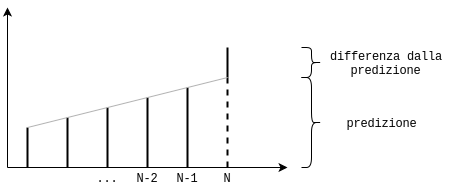
\includegraphics[width=9cm]{./Images/7.1.png}
\end{figure}
\FloatBarrier

\end{comment}